
\chapter{SOLUTION}

% breadth-first explanation, examples inside protocol, explain only in context of Tor

% relative vs against

\section{Overview}

We propose the Onion Name Service, or OnioNS, a system which uses enables transparent translation of .tor domain names to .onion addresses. The system has three main aspects: the generation of self-signed claims on domain names by hidden service operators, the processing of domain information within the OnioNS servers, and the receiving and authentication of domain names by a Tor client.

First, a hidden service operator, Bob, generates an association claim between a meaningful domain name and a .onion address. Without loss of generality, let this be example.tor $ \rightarrow $ example0uyw6wgve.onion. For security reasons we do not introduce a central repository and authority from which Bob can purchase domain names; however, domains are not trivially obtainable and Bob must expend effort to claim and maintain ownership of example.tor. We achieve this through a proof-of-work scheme. Proof-of-work systems are noteworthy for their asymmetry: they require the issuer to spend effort to find an answer to a moderately hard computational problem, but once solved can be easily verified correct by any recipient. The requirement of proof-of-work fulfils three main purposes:

\begin{enumerate}
	\item Significantly reduces the threat of record flooding.
	\item Introduces a barrier-of-entry that encourages the utilization of domain names and the availability of the underlying hidden services.
	\item Increases the difficulty of domain squatting, a denial-of-service attack where a third-party claims one or more valuable domain names for the purpose of denying or selling them en masse to others. In Tor's anonymous environment, this vector is particularly prone to Sybil attacks.
\end{enumerate}

Bob then digitally signs his association and the proof-of-work with his service's private key.

Second, Bob uses a Tor circuit to anonymously transmit his association, proof-of-work, digital signature, and public key to OnioNS nodes, a subset of Tor routers. This set is deterministically derived from the volatile Tor consensus documents and is rotated periodically. The OnioNS nodes receive Bob's information, distribute it amongst themselves, and later archive it in a sequential transaction database, of which each OnioNS node holds their own copy. The nodes also digitally sign this database and distribute their signatures to the other nodes. Thus the OnioNS Tor nodes maintain a common database and have each vouched for its authenticity.

Third, a Tor client, Alice, uses a Tor client to anonymously connect to one of these OnioNS nodes and request a domain name. Without loss of generality, let this request be example.tor. Alice receives Bob's ``example.tor $ \rightarrow $ example0uyw6wgve.onion'' association, his proof-of-work, his digital signature, and his public key. Alice then verifies the proof-of-work and Bob's signature against his public key, and hashes his key to confirm the accuracy of example0uyw6wgve.onion. Alice then looks up example0uyw6wgve.onion in Tor's distributed hashtable, finds Bob's introduction point, and confirms that its knowledge of Bob's public key matches the key she received from the OnioNS nodes. Finally, she finishes the Tor hidden service protocol and begins communication with Bob. In this way, Alice can contact Bob through his chosen domain name without resorting to use lower-level hidden service addresses. The uniqueness and authenticity of the Bob's domain name is maintained by the subset of Tor nodes.

%At a high level, OnionNS' master page-chain is maintained by a randomly-selected rotating set of high-capacity Tor nodes. Other Tor nodes may mirror the page-chain, distributing the load and responsibilities across the network. The system supports a variety of command and control operations including Create, Domain Query, Onion Query, Modify, Move, Renew, and Delete.

% node vs server

% capitalize nouns that are defined

\section{Definitions}

To discuss OnioNS precisely we must first define some central terms that we will use throughout the rest of this document. We detail their exact contents in section \ref{sec:DataStructures} and how they are used throughout sections \ref{sec:BasicDesign} and \ref{sec:Protocols}.

\begin{description}
	\item[domain name] \hfill \\
		A \emph{domain name} is a case-insensitive identification string claimed by a hidden service operator. The syntax of OnioNS domain names mirrors the Clearnet DNS; we use a sequence of name-delimiter pairs with the .tor Top Level Domain (TLD). The TLD is a name at depth one and is preceded by names at sequentially increasing depth. The term ``domain name'' refers to the identiciation string as a whole, while ``second-level domain'' refers to the central name that is immediately followed by the TLD, as illustrated in Figure \ref{fig:sampleDomain}. Domain names point to \emph{destinations} -- other domain names with either the .tor or .onion TLD.
		
		\begin{figure}[htbp]
			\centering
			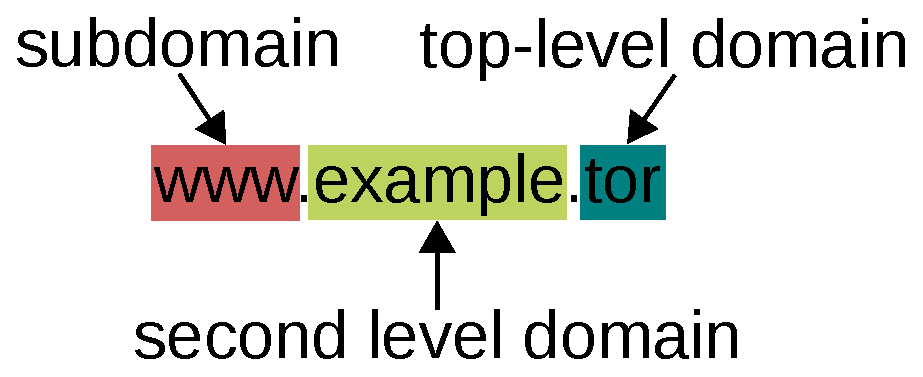
\includegraphics[width=0.5\textwidth]{images/domain-name.eps}
			\caption{A sample domain name: a sequence of labels separated by delimiters. In OnioNS, hidden service operators build associations between second-level domain names and their hidden service address.}
			\label{fig:sampleDomain}
		\end{figure}
		
	The Clearnet DNS defines a hierarchy of administrative realms that are closely tied to the depth of each name. By contrast, OnioNS makes no such distinction; we let hidden service operators claim second-level names and then control all names of greater depth under that second-level name. Hidden service operators may then choose to administer or sell the use of their subdomains, but this is outside the scope of this project.

	\item[Record] \hfill \\
		A \emph{Record} is a small textual data structure that contains one or more domain-destination pairs, a proof-of-work, a digital signature, and a public key. Records are issued by hidden service operators and sent to OnioNS servers. Every Record is self-signed with the hidden service's key. In section \ref{sec:Record} we describe the five different types of Records: Create, Modify, Move, Renew, and Delete. A Create Record represents a registration on an unclaimed second-level domain name, Modify, Move, and Renew are operations on that domain name or its subdomains, and a Delete Record relinquishes ownership over the second-level domain name and all its subdomains.
		
	\item[broadcast] \hfill \\
		The term for the protocol described in section \ref{sec:ProtoHiddenServices} that describes the uploading of new Records to OnioNS servers through Tor circuits and then the subsequent confirmation that the Record has been received.
		
	\item[Snapshot] \hfill \\
		A \emph{Snapshot} is textual database designed to hold collections of Records in a short-term volatile cache. They are also used to transmit sets of Records between OnioNS servers.

	\item[Page] \hfill \\
		A \emph{Page} is textual database designed to archive one or more Records in long-term storage. Pages are held and digitally signed by OnioNS nodes and are writable only for fixed periods of time before they are read-only. Each Page contains a link to a previous Page, forming an append-only public ledger known as an \emph{Pagechain}. This forms a two dimensional distributed data structure: the chain of Pages grows over time and there are multiple redundant copies of each Page spread out across the network at any given time. 
		
	\item[Mirror] \hfill \\
		A \emph{Mirror} is any machine (inside or outside of the Tor network) that has performed a synchronization (section \ref{sec:Synchronization}) against the OnioNS network and now holds a complete copy of the Pagechain. Mirrors do not actively participate in the OnioNS network and do not have the power to manipulate the central page-chain.

	\item[Quorum Candidate] \hfill \\
		A \emph{Quorum Candidates} are \emph{Mirrors} inside the Tor network that have also fulfilled two additional requirements: 1) they must demonstrate that they are an up-to-date Mirror, and 2) that they have sufficient CPU and bandwidth capabilities to handle powering OnioNS in addition to their regular Tor duties. In other words, they are qualified and capable to power OnioNS, but have not yet been chosen to do so.
		
	\item[Quorum] \hfill \\
		A \emph{Quorum} is a subset of Quorum Candidates who have active responsibility over maintaining the master OnioNS Pagechain. Each Quorum node actively its own Page, which has a lifetime of that Quorum. The Quorum is randomly chosen from Quorum Candidates as described in section \ref{sec:ProtoTorClients}.
					
	\item[flood] \hfill \\
		The term for the periodic burst of communication that occurs between Quorum nodes wherein Snapshots are exchanged and each Quorum node obtains the state and digital signature of the current Page maintained by all other Quorum nodes. This communication is described in section \ref{sec:ProtoOnioNServers}.
\end{description}

\begin{figure}[htbp]
	\centering
	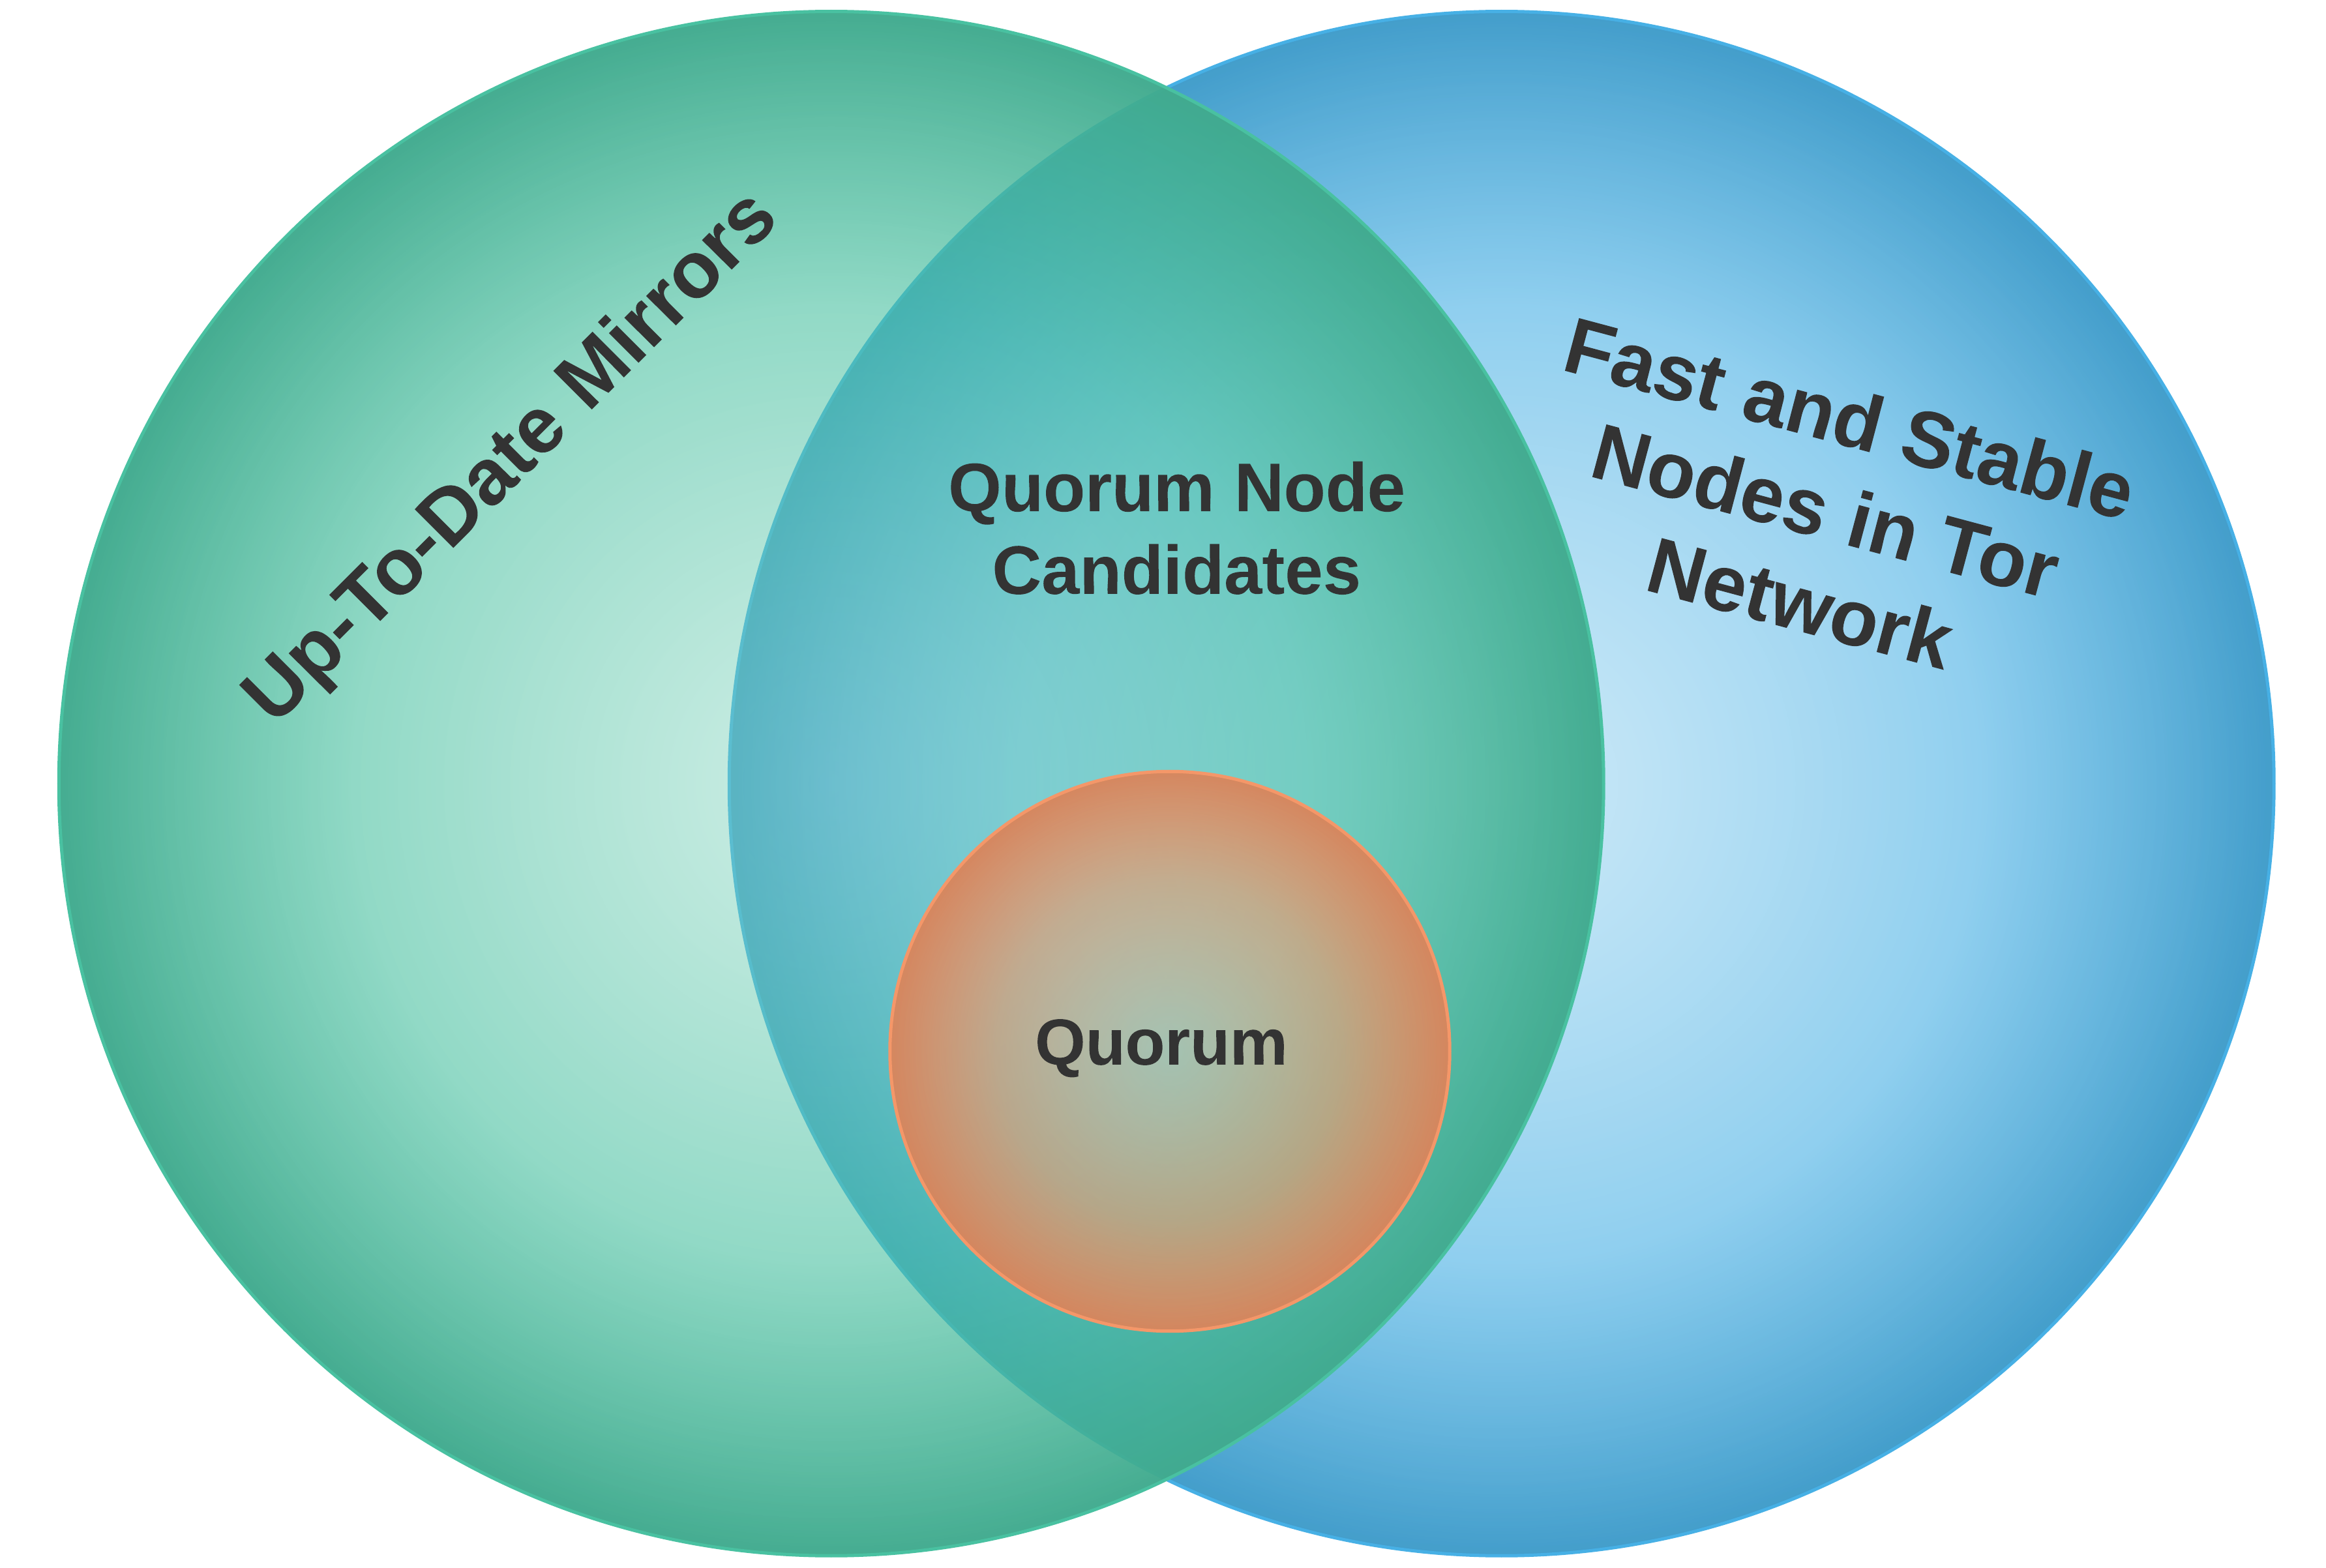
\includegraphics[width=0.5\textwidth]{images/LucidCharts/Participants.png}
	\caption{The relationship between Mirrors, Quorum Candidates, and the Quorum. A Mirror is any machine that holds the OnioNS Pagechain, Quorum Candidates are both up-to-date Mirrors and reliable Tor nodes, and the Quorum is randomly selected from the pool of Quorum Candidates.}
\end{figure}

Throughout the rest of this document, let Alice be a Tor client, and Bob be the operator of a hidden service. Assume that neither Alice nor Bob run Tor relays themselves, but let them only use Tor. Therefore Alice and Bob know the public keys of the Tor authority nodes and they can obtain and fully verify any past or current set of consensus documents. Bob has access to his hidden service private RSA key and may or may not have a PGP key with a subkey for email encryption.

\section{Basic Design}
\label{sec:BasicDesign}

OnioNS is build on a fundamental sequence of operations, as illustrated in Figure \ref{fig:basicDesign}:

\begin{enumerate}
	\item Bob generates a valid Record.
	\item Bob broadcasts the Record to the Quorum.
	\item The Record is flooded across the Quorum.
	\item Each Quorum node stores the Record into its current Page at the head of its local Pagechain.
	\item Alice queries the system for a domain name.
	\item Alice receives back the Record matching that domain name and confirms its validity.
	\item Alice connects to Bob via the hidden service protocol.
\end{enumerate}

These steps describe the propagation of any Record throughout the entire network. The protocols for each party are described in sections \ref{sec:ProtoHiddenServices}, \ref{sec:ProtoOnioNServers}, and \ref{sec:ProtoTorClients}, respectively. It should be noted that the activities of Alice, Bob, and the Quorum occur asynchronously: hidden service operator may be transmitting Records to the Quorum at the same time that clients are querying for other domain names.

\begin{figure}[htbp]
	\centering
	\begin{tikzpicture}[->, node distance=2.4cm, main node/.style={circle, fill=blue!20, draw, font=\sffamily\bfseries}]

			\node[main node] (1) {$ R_{G} $};
			\node[main node] (2) [right of=1] {};
			\node[main node] (3) [right of=2] {Alice};
			\node[main node] (4) [right of=3] {};

			\node[main node] (5) [below of=1] {$ R_{E} $};
			\node[main node] (6) [right of=5] {$ R_{M} $};
			\node[main node] (7) [right of=6] {};
			\node[main node] (8) [right of=7] {};

			\node[main node] (9) [below of=5] {};
			\node[main node] (10) [right of=9] {OnioNS};
			\node[main node] (11) [right of=10] {};
			\node[main node] (12) [right of=11] {$ R_{E} $};

			\node[main node] (13) [below of=9] {};
			\node[main node] (14) [right of=13] {$ R_{M} $};
			\node[main node] (15) [right of=14] {$ R_{G} $};
			\node[main node] (16) [right of=15] {Bob};

			% Alice-OnioNS conversation
			\tikzstyle{EdgeStyle}=[bend right, -, green]
			\Edge[](3)(1)
			\tikzstyle{EdgeStyle}=[bend left=15, -, green]
			\Edge[](1)(6)
			\Edge[](5)(6)
			\draw[thick, ->, red, postaction={decorate, decoration={text along path, text align=center, text={Query}, raise=4pt}}] (5) to [bend left=10] (10){};
			\draw[thick, <-, blue, postaction={decorate, decoration={text along path, text align=center, text={Response}, raise=-9pt}}] (5) to [bend right=10] (10){};

			% Bob-OnioNS conversation
			\tikzstyle{EdgeStyle}=[bend right=15, -, green]
			\Edge[](16)(15)
			\Edge[](15)(14)
			\tikzstyle{EdgeStyle}=[bend left=12, -, green]
			\Edge[](14)(12)
			\draw[thick, red, <-, postaction={decorate, decoration={text along path, text align=center, text={Record}, raise=3pt}}] (10) to [bend left=40] (12){};
			\draw[thick, blue, ->, postaction={decorate, decoration={text along path, text align=center, text={Confirmation}, raise=-10pt}}] (10) to [bend left=30] (12){};

		\end{tikzpicture}
	\caption{Bob uses a Tor circuit (guard, middle, and exit Tor routers) to anonymously broadcast a record to OnioNS. Alice uses her own Tor circuit to query the system for a domain name, and she is given Bob's record in response. Then Alice connects to Bob by Tor's hidden service protocol (section \ref{sec:HiddenServices}).}
	\label{fig:basicDesign}
\end{figure}

\subsection{Domain Name Operations}

Bob first generates a valid Record which he transmits over a Tor circuit to a randomly-selected Quorum node, who confirms acceptance or returns an error message otherwise. Bob's Record is flooded to the rest of Quorum via the periodic flushing of Snapshots by each Quorum node. Therefore, Bob can confirm that the rest of the Quorum received his Record by constructing another circuit to a different randomly-selected Quorum node and asking it for his Record. This process is illustrated in Figure \ref{fig:recordBroadcast}.

\begin{figure}[htbp]
	\centering
	\begin{tikzpicture}[->, node distance=2.4cm, main node/.style={circle, fill=blue!20, draw, font=\sffamily\bfseries}]

			\node[main node] (1) {$ Q_{1} $};
			\node[main node] (2) [right of=1] {$ Q_{2} $};
			\node[main node] (3) [right of=2] {};
			\node[main node] (4) [right of=3] {$ Q_{3} $};

			\node[main node] (5) [below of=1] {};
			\node[main node] (6) [right of=5] {$ Q_{4} $};
			\node[main node] (7) [right of=6] {};
			\node[main node] (8) [right of=7] {};

			\node[main node] (9) [below of=5] {$ R_{M} $};
			\node[main node] (10) [right of=9] {};
			\node[main node] (11) [right of=10] {$ R_{E} $};
			\node[main node] (12) [right of=11] {$ Q_{5} $};

			\node[main node] (13) [below of=9] {};
			\node[main node] (14) [right of=13] {};
			\node[main node] (15) [right of=14] {$ R_{E} $};
			\node[main node] (16) [right of=15] {HS};

			% draw 1st and 2nd part of circuit
			\tikzstyle{EdgeStyle}=[bend right=12, -, green]
			\Edge[](16)(15)
			\Edge[](9)(15)

			% draw last part of circuit
			\tikzstyle{EdgeStyle}=[bend left=17, -, green]
			\Edge[](9)(11)

			% draw record moving from exit to 1st q. node
			\draw[thick, red, <-, postaction={decorate, decoration={text along path, text align=center, text={Record}, raise=3pt}}] (6) to [bend right=15] (11){};

			% draw verification with second q. node
			\draw[thick, red, ->, postaction={decorate}] (12) to [bend left=15] (11){};

			% draw upper left propegation
			\tikzstyle{EdgeStyle}=[bend left=12, ->, blue]
			\Edge[](6)(2)
			\Edge[](6)(1)

			% draw upper right propegation
			\tikzstyle{EdgeStyle}=[bend left=20, ->, blue]
			\Edge[](6)(12)
			\draw[thick, blue, postaction={decorate, decoration={text along path, text align=center, text={Snapshot}, raise=3pt}}] (6) to [bend right=18] (4){};

		\end{tikzpicture}
	\caption{Bob uses his existing circuit (green) to inform \emph{quorum} node $ Q_{4} $ of the new record. $ Q_{4} $ then floods it via \emph{Snapshots} to all other \emph{Quorum} nodes. Each node stores it in their own \emph{Page} for long-term storage. Bob confirms from another \emph{Quorum} node $ Q_{5} $ that his Record has been received.}
	\label{fig:recordBroadcast}
\end{figure}

\subsection{Pagechain Maintenance}

The Pagechain is OnioNS' fundamental data structure and is the central component of the entire system. It is a distributed append-only transactional database of a fixed maximum length. Each Page references a previous Page, forming a long chain. The head of the chain (the latest Page) is maintained and digitally signed by each member of the current Quorum. The Pagechain is designed as a public and fully confirmable data structure -- that is, any Mirror can check the integrity of each Page and the Records contained within them, the uniqueness of domain names, and the validity of the digital signatures on each Page from all Quorum nodes.

Any Mirror may continue its own Pagechain by generating a new Page, adding that Page to the front of its Pagechain, deleting the oldest Page, and then merging new Records into the new Pagechain head. When a Quorum Candidate is chosen as a Quorum node, it modifies its local Pagechain in this way. Assuming that the entire Quorum is honest and maintains perfect flooding communication, the entire Quorum would be in agreement. However, any Quorum node may experience downtime and may miss Snapshot broadcasts, have data corruption, act maliciously, or have other cause for its Pagechain head to deviate relative to the others. Therefore, disagreements may inevitably form within the Quorum. We address this under our original assumption that the largest set of Quorum nodes that have matching and valid Pagechains are also acting honestly. Therefore each Mirror can follow this rule to derive the master Pagechain and safely ignore any ``sidechains''. Likewise, each new honest Quorum member follows suite when creating a new Page, as described in section \ref{sec:ProtoOnioNServers}. Thus the Pagechain is at least partially self-healing. We illustrate this in Figure \ref{fig:sidechains}.

\begin{figure}[htbp]
	\centering
	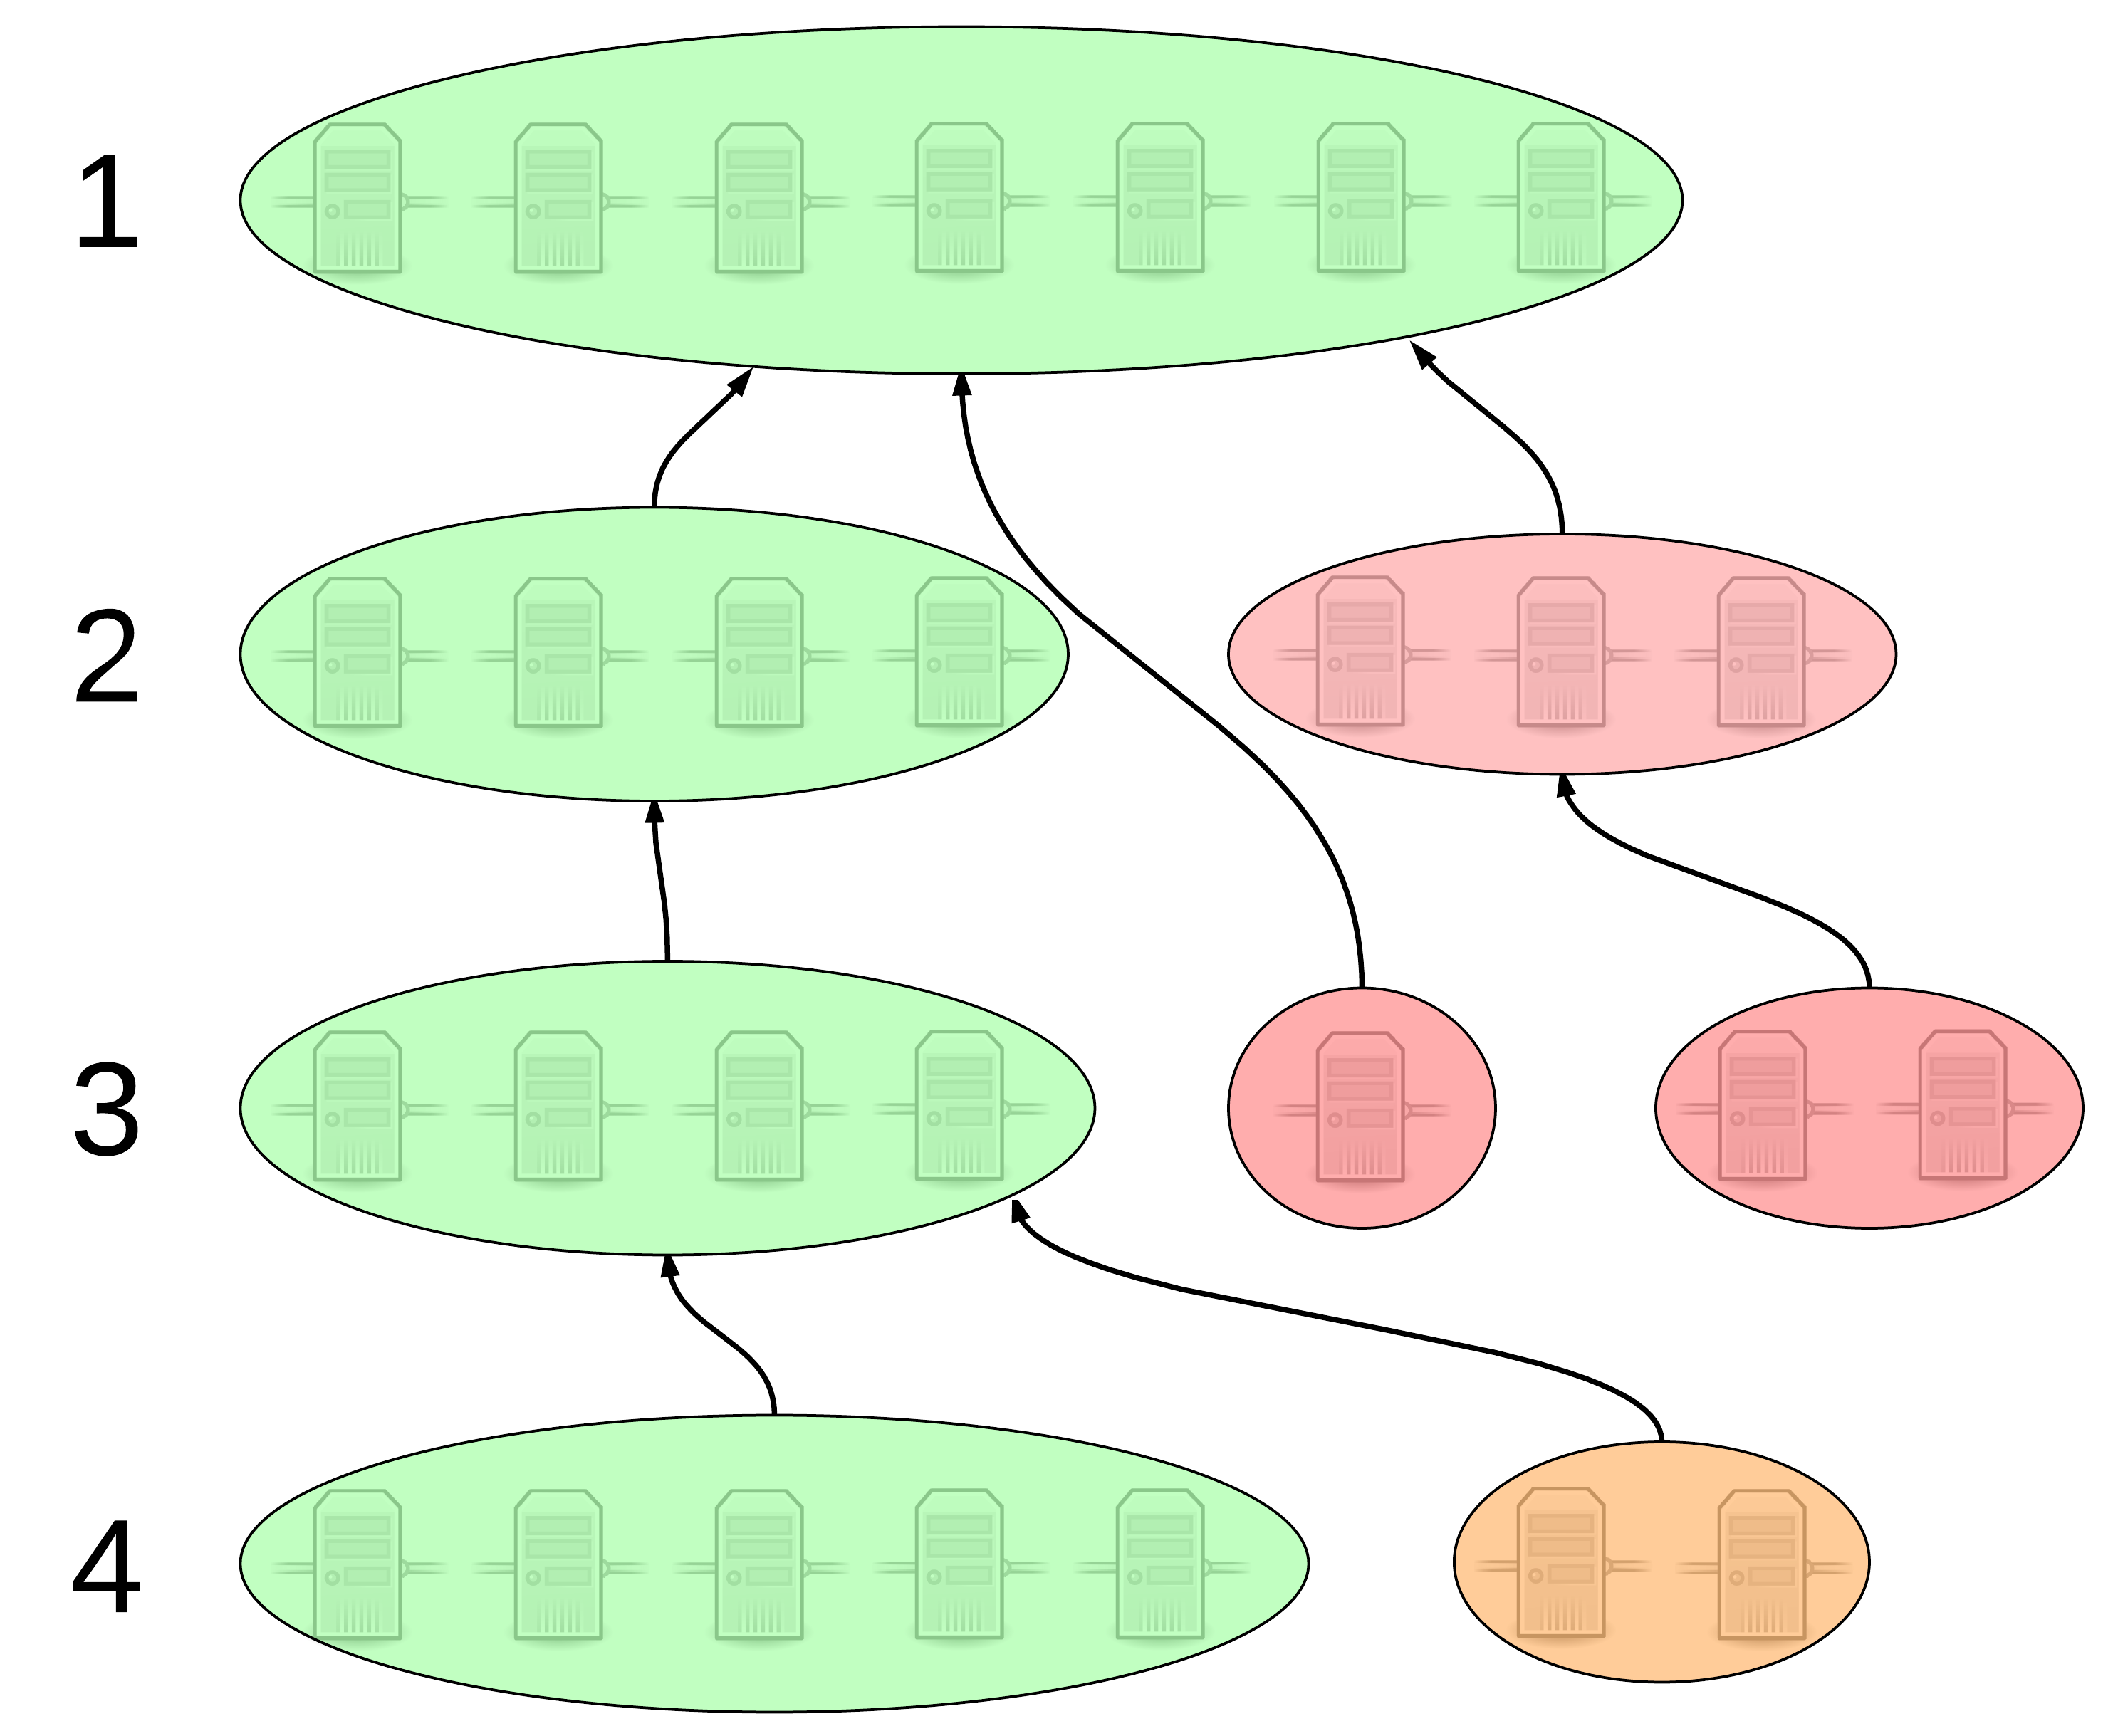
\includegraphics[width=0.65\textwidth]{images/LucidCharts/Page-chain.png}
	\caption{An example Pagechain across four Quorums. Each Page contains a references to a previous Page, forming a distributed append-only chain. $ \mathrm{Quorum}_{1} $ is honest and maintains reliable flooding communication, and thus has identical Pages. $ \mathrm{Quorum}_{2} $'s largest cluster is likewise in agreement, but there are three nodes which are acting maliciously together and have changed their Pages. Node 5 in $ \mathrm{Quorum}_{3} $ references an old page in attempt to bypass $ \mathrm{Quorum}_{2} $'s records, and nodes 6-7 are colluding with nodes 5-7 from $ \mathrm{Quorum}_{2} $. Finally, $ \mathrm{Quorum}_{4} $ has two nodes that acted honestly but did not record new records, so their Pagechains differ from the others. However, across all four days the largest clusters are honest nodes and thus integrity remains in the master Pagechain.}
	\label{fig:sidechains}
\end{figure}

\subsection{Client Request}

% todo: make diagram of this

Let Bob and Charlie be two hidden services, and assume that OnioNS knows a Record from Bob containing an ``example.tor $ \rightarrow $ example0uyw6wgve.onion'' association, and a Record from Charlie containing ``example2.tor $ \rightarrow $ example5chqt7to6.onion, sub.example2.tor $ \rightarrow $ example.tor''. Now let Alice request ``sub.example2.tor''.

Since the .tor TLD is not used by the Clearnet DNS, Alice's client software must direct the request through a Tor circuit to some OnioNS resolver, $ O_{r} $. By default, $ O_{r} $ belongs to the set of Quorum Candidate nodes although Alice may override this and choose some Mirror if she wishes. For security and load reasons, Quorum nodes refuse to respond to queries, so Alice cannot ask them. Following Alice's request, $ O_{r} $ searches its local Pagechain for ``example2.tor'' and finds Charlie's Record, which it then sends to Alice. Alice sees the ``sub.example2.tor $ \rightarrow $ example.tor'' association and now queries $ O_{r} $ for ``example.tor''. $ O_{r} $ then locates and sends Bob's Record to Alice. Alice sees that ``example.tor'' has a destination of ``example0uyw6wgve.onion'', and because it has a .onion address she does not need to issue any more queries. Instead, Alice connects to Bob's example0uyw6wgve.onion service via the Tor  hidden service protocol and sends her original request (``sub.example2.tor'') to Bob. As is the case with the Clearnet, Bob's web server may or may not provide specific content to Alice based on this request, but his configuration is outside our scope.

In this way, Alice can query an OnioNS resolver for some Charlie-selected domain name and recursively resolve it to a .onion address transparently. The number of resolutions Alice makes is fixed to a maximal length (section \ref{sec:Record}) so this algorithm always completes. We discuss minor optimizations and security enhancements to this procedure in section \ref{sec:ProtoTorClients}.

\section{Primitives}

\subsection{Cryptographic}

OnionNS makes use of cryptographic hash algorithms, digital signatures, proof-of-work, and a pseudorandom number generator.

\begin{itemize}
	\item Let $ H(x) $ be a cryptographic hash function. In our reference implementation we define $ H(x) $ as SHA-384, a truncated and slight modificated derivative of SHA-512. Currently the best preimage attack of SHA-512 breaks 57 out of 80 rounds in $ 2^{511} $ time.\cite{li2012converting} SHA-384 is included in the National Security Agency's Suite B Cryptography for protecting information classified up to Top Secret.
	\item Let $ S_{d}(m, r) $ be a deterministic RSA digital signature function that accepts a message $ m $ and a private RSA key $ r $ and returns an RSA digital signature. Let $ S_{d}(m, r) $ use $ H(x) $ as a digest function on $ m $ in all use cases. In our reference implementation we define $ S_{d}(m, r) $ as EMSA-PSS, (EMSA4) a probabilistic signature scheme defined by PKCS1 v2.1 and republished in 2003's RFC 3447.
	\item Let $ S_{p}(m, r) $ be $ S_{d}(m, r) $ but with probabilistic output. We suggest EMSA-PKCS1-v1.5, (EMSA3) defined by 1998's RFC 2315.
	\item Let $ S_{\mathit{ed}}(m, c) $ be an Ed25519 digital signature function that accepts a message $ m $ and a private Curve25519 key $ c $ and returns a 64-byte Ed25519 digital signature. Ed25519 is digital signature scheme designed with high performance, strong implementation security, and minimal keypair and signature sizes objectives in mind. The Ed25519 elliptic curve is birationally equivalent to Curve25519, and Curve25519 keys can be converted to Ed25519 keys in $ \mathcal{O}(1) $ time.\cite{bernstein2011high} Let $ S_{\mathit{ed}}(m, c) $ use $ H(x) $ as a digest function on $ m $ in all use cases.
	\item Let $ \mathrm{PoW}(i) $ be a proof-of-work scheme such as a strong key derivation function that accepts an input key $ k $ and returns a derived key. Our reference implementation uses a fixed salt and scrypt, a password-based key derivation function which is notable for its large memory and CPU requirements during its operation. The scrypt function provides significantly greater resistance to custom hardware attacks and massively parallel computation primarily due to its memory requirements. This limits attackers to the same software implementation and asymptotic cost as legitimate users.\cite{percival2009stronger}\cite{percival2012scrypt} We choose scrypt because of these advantages over other key derivation functions such as SHA-256 or PBKDF2. For these reasons scrypt is also common for proof-of-work purposes in some cryptocurrencies such as Litecoin.
	\item Let $ \mathit{R}(s) $ be a pseudorandom number generator that accepts an initial seed $ s $ and returns a list of numerical pseudorandom numbers. We suggest MT19937, commonly known as the Mersenne Twister. This generator is widely used throughout most programming languages and is well known for its speed, long period, and the high quality of its pseudorandom output, although it is not cryptographically secure.\cite{matsumoto1998mersenne}
\end{itemize}

\subsection{Symbols}

\begin{itemize}
	\item Let $ L_{Q} $ represent size of the Quorum.
	\item Let $ L_{T} $ represent the number of routers in the Tor network.
	\item Let $ q $ be an Quorum iteration counter.
	\item Let $ \Delta q $ be the lifetime of a Quorum in days: every $ \Delta q $ days $ q $ is incremented by one and a new Quorum is chosen.
	\item Let $ s $ be a Snapshot iteration counter.
	\item Let $ \Delta s $ be the lifetime of a Snapshot in days: every $ \Delta s $ minutes $ s $ is incremented by one, a flood happens, and a fresh Snapshot is used.
\end{itemize}

All textual databases are encoded in JSON. JSON is significantly more compact than XML, but retains readability. Its support of basic primitive types is highly applicable to our needs. Additionally, we consider the JSON format safer than byte-level encoding.

\section{Data Structures}
\label{sec:DataStructures}

\subsection{Record}
\label{sec:Record}

There are five different types of Records: Create, Modify, Move, Renew, and Delete. The latter four Records mimic the format of the Create Record with minor exceptions.

\subsubsection{Create}

A Create record consists of nine components: \emph{type}, \emph{nameList}, \emph{contact}, \emph{timestamp}, \emph{consensusHash}, \emph{nonce}, \emph{pow}, \emph{recordSig}, and \emph{pubHSKey}. Fields that are optional are blank unless specified, and all fields are encoded in base64, except for \emph{nameList} and \emph{timestamp}, which are encoded in standard UTF-8.

\renewcommand{\arraystretch}{1.75} % increase spacing between columns
\begin{center}
    \begin{longtabu}{ | l | c | p{9.5cm} |}
    \hline
    \textbf{Field} & \textbf{Required?} & \textbf{Description} \\
    type & Yes & A textual label containing the type of Record. In this case, \emph{type} is set to ``Create''. \\
    nameList & Yes & An array list of domain names and their destinations. The list of domain names includes one or more second-level domain name, while the remainder of the list contains zero or more subdomains (names at level $ < 2 $) under that second-level domains. In this way, records can be referenced by their unique second-level domain names. Destinations use either .tor or .onion TLDs. \\
    contact & No & Bob's PGP key fingerprint, if he has a key and chooses to disclose it. If the fingerprint is listed, clients may query a public keyserver for this fingerprint, obtain the PGP public key, and contact Bob over encrypted email. \\
    timestamp & Yes & The UNIX timestamp of when the issuer created the registration and began $ \mathrm{PoW}(i) $. \\
    consensusHash & Yes & The hash of the consensus document that generated $ \mathit{Quorum}_{q} $ \\
    nonce & Yes & Four bytes that serve as a source of randomness for $ \mathrm{PoW}(i) $. \\
   	pow & Yes & 16 bytes that store the output of $ \mathrm{PoW}(i) $. \\
   	recordSig & Yes & The output of $ S_{p}(m, r) $ where $ m = \mathit{nameList} \concat \mathit{timestamp} \concat \mathit{consensusHash} \concat \mathit{nonce} \concat \mathit{pow} $ and $ r $ is the hidden service's private RSA key. \\
   	pubHSKey & Yes & Bob's public RSA key. \\
    \hline
    \caption{A Create record, which contains fields common to all records. Every record is self-signed and must have verifiable proof-of-work before it is considered valid.}
    \end{longtabu}
\end{center}

\subsubsection{Modify}

A Modify record allows an owner to update his registration with updated information. The Modify record has identical fields to Create, but \emph{type} is set to ``Modify''. The owner corrects the fields, updates \emph{timestamp} and \emph{consensusHash}, revalidates the proof-of-work, and transmits the record. Modify records have a difficulty of $ \frac{\textrm{difficulty}_{\textrm{Create}}}{4} $. Modify records can be used to add and remove domain names but cannot be used to claim additional second-level domains.

\subsubsection{Move}

% prevents the seller from selling modified records and forcing the buyer to issue a Modify record

A Move record is used to transfer one or more second-level domain names and all associated subdomains from one owner to another. Move records have all the fields of a Create record, have their \emph{type} is set to ``Move'', and contain two additional fields: \emph{target}, a list of domain-destination pairs, and \emph{destPubKey}, the public key of the new owner. Domain names and their destinations contained in \emph{target} cannot be modified; they must match the latest Create, Renew, or Modify record that defined them. Move records also have a difficulty of $ \frac{\textrm{difficulty}_{\textrm{Create}}}{4} $.

\subsubsection{Renew}

% put "page" in italics everywhere?

Second-level domain names (and their associated domain names) expire every $ L $ days because (as explained below) the page-chain has a maximum length of $ L $ pages. Renew records must be reissued periodically at least every $ L $ days to ensure continued ownership of domain names. Renew records are identical to Create records, except that \emph{type} is set to ``Renew''. No modifications to existing domain names can be made in Renew records, and the domain names contained within must already exist in the page-chain. Similar to the Modify and Move records, Renew records have a difficulty of $ \frac{\textrm{difficulty}_{\textrm{Create}}}{4} $.

\subsubsection{Delete}

% attacker could compromise key, issues Move record before original owner knew of compromise. Or attacker could then reclaim domain name

If a owner's private key is compromised or if they wish to relinquish ownership rights over all of their domain names, they can issue a Delete record. Aside from their \emph{type} field set to ``Delete'', Delete records are identical in form to Create records but have the opposite effect: all second-level domains contained within the record are purged from local caches and made available for others to claim. There is no difficulty associated with Delete records, so they can be issued instantly.

\subsection{Snapshot}

Snapshots contain four fields: \emph{originTime}, \emph{recentRecords}, \emph{fingerprint}, and \emph{snapshotSig}.

\begin{description}
	\item[originTime] \hfill \\
		Unix time when the snapshot was first created.
	\item[recentRecords] \hfill \\
		A array list of records in reverse chronological order by receive time.
	\item[fingerprint] \hfill \\
		The hash of the public key of the machine maintaining this snapshot. This is the Tor fingerprint, a unique identification string widely used throughout Tor infrastructure and third-party tools to refer to specific Tor nodes.
	\item[snapshotSig] \hfill \\
		The output of $ S_{\mathit{ed}}(\mathit{originTime} \concat \mathit{recentRecords} \concat \mathit{fingerprint}], c) $ where $ c $ is the machine's private Curve25519 NTor key.
\end{description}

\emph{snapshotSig} is 
		
\subsection{Page}

Each page contains five fields, \emph{prevHash}, \emph{recordList}, \emph{consensusDocHash}, \emph{fingerprint}, and \emph{pageSig}.

\begin{description}
	\item[prevHash] \hfill \\
		The SHA-384 hash of \emph{prevHash}, \emph{recordList}, and \emph{consensusDocHash} of a previous page.
	\item[recordList] \hfill \\
		An array list of records, sorted in a deterministic manner.
	\item[consensusDocHash] \hfill \\
		The SHA-384 of $ cd $.
	\item[fingerprint] \hfill \\
		The hash of the public key of the machine maintaining this page, the Tor fingerprint.
	\item[pageSig] \hfill \\
		The output of $ S_{\mathit{ed}}(H(\mathit{prevHash} \concat \mathit{recordList} \concat \mathit{consensusDocHash})], c) $ where $ c $ is the machine's private Curve25519 NTor key.
\end{description}	
		
\section{Protocols}
\label{sec:Protocols}

% todo: the examples here aren't valid

\subsection{Hidden Services}
\label{sec:ProtoHiddenServices}

\subsubsection{Record Generation}

Mirrors and Tor clients check the validity of Records that they receive through synchronization or query responses, respectively. Invalid Records will be rejected by all parties, so Bob must generate a valid Record before broadcast.

\begin{enumerate}
	\item Bob selects the value for \emph{type} based on the desired operation.
	\item Bob constructs the \emph{nameList} domain-destination associations.
	\item Bob provides his PGP key fingerprint in \emph{contact} or leaves it blank if he doesn't have a PGP key or if he chooses not to disclose it. Bob can derive his PGP fingerprint with the ``gpg --fingerprint'' Unix command.
	\item Bob records the number of seconds since the Unix epoch in \emph{timestamp}.
	\item Bob sets \emph{consensusHash} to the output of $ H(x) $, where $ x $ is the consensus document published at 00:00 GMT on day $ \floor[\big]{\frac{q}{\Delta q}} $.
	\item Bob initially defines \emph{nonce} as four zeros.
	\item Let $ \mathit{central} $ be $\mathit{type} \concat \mathit{nameList} \concat \mathit{contact} \concat \mathit{timestamp} \concat \mathit{consensusHash} \concat \mathit{nonce} $.
	\item Bob sets \emph{pow} as $ \mathrm{PoW}(\mathit{central}) $.
	\item Bob sets \emph{recordSig} as the output of $ S_{d}(m, r) $ where $ m = \mathit{central} \concat \mathit{pow} $ and $ r $ is Bob's private RSA key.
	\item Bob saves the PKCS.1 DER encoding of his RSA public key in \emph{pubHSKey}.
\end{enumerate}

Bob then must increment \emph{nonce} and reset \emph{pow} and \emph{recordSig} until $ H(\mathit{central} \concat \mathit{pow} \concat \mathit{recordSig}) \leq 2^{\mathit{difficulty} * \mathit{count}} $ where \emph{difficulty} is a fixed constant that specifies the work difficulty and \emph{count} is the number of second-level domain names claimed in the Record. An example of a completed and valid record is shown in Figure \ref{fig:sampleRecord}.

\begin{figure}
	\begin{lstlisting}
	{
		"names": {
			"example.tor": "exampleruyw6wgve.onion"
		}
		"contact": "AD97364FC20BEC80",
		"timestamp": 1424045024,
		"consensusHash": "uU0nuZNNPgilLlLX2n2r+sSE7+N6U4DukIj3rOLvzek=",
		"nonce": "AAAABw==",
		"pow": "4I4dzaBwi4AIZW8s2m0hQQ==",
		"recordSig": 	"KSaOfzrXIZclHFcYxI+3jBwLs943wxVv3npI5ccY/kBEpyXRSopzjoFs746n0tJqUpdY4Kbe6DBwERaN7ELmSSK9Pu6q8QeKzNAh+QOnKl0fKBN7fqowjkQ3ktFkR0Vuox9WrrbNTMa4+up0Np52hlbKA3zSRz4fbR9NVlh6uuQ=",
		"pubHSKey": "MIGhMA0GCSqGSIb3DQEBAQUAA4GPADCBiwKBgQDE7CP/kgwtJhTTc4JpuPkvA7Ln9wgc+fgTKgkyUp1zusxgUAn1c1MGx4YhO42KPB7dyZOf3pcRk94XsYFY1ULkF2+tf9KdNe7GFzJyMFCQENnUcVXbcwLH4vAeiGK7R/nScbCbyc9LT+VE1fbKchTL1QzLVBLqJTxhR+9YPi8x+QIFAdZ8BJs="
	}
	\end{lstlisting}
	\caption{A sample registration record. The textual fields are in UTF-8, while the binary fields are in base64. The structure is encoded in JSON.}
	\label{fig:sampleRecord}
\end{figure}

\subsubsection{Record Validation}

Let Carol be a Tor client or a Mirror that receives a Record from another Mirror. Bob must also perform these procedures to ensure that he sends a valid Record.

\begin{enumerate}
	\item Carol checks that the Record contains valid JSON.
	\item Carol checks that \emph{type} is either ``Create'', ``Modify'', ``Move'', ``Renew'', or ``Delete''.
	\item Carol checks that \emph{nameList} is has a length $ \in [1,24] $, contains at least one second-level domain name, and that all subdomains have a second-level domain name within \emph{nameList}. Additionally, Carol checks that there is no domain name nor destination that uses more than 16 names, that is longer than 32 characters, or whose total length is more than 128 characters.
	\item Carol checks that \emph{contact} is either 0, 16, 24, or 32 characters in length, and that \emph{contact} is valid hexadecimal.
	\item Carol checks that \emph{timestamp} is not in the future nor more than 48 hours old relative to her system clock.
	\item Carol checks that \emph{pubHSKey} is a valid PKCS.1 DER-encoded public 1024-bit RSA key, and that when converted to a .onion address that address appears at least once in \emph{nameList}.
	\item Carol checks the validity of \emph{recordSig} deterministic signature against \emph{pubHSKey} and $ \mathit{central} \concat \mathit{pow} $.
	\item Carol obtains the $ \floor[\big]{\frac{q}{\Delta q}} $ 00:00 GMT consensus document and checks $ H(x) $ on it against \emph{consensusHash}. She also confirms that the consensus document is no older than $ \mathrm{min}(48, 12 * \Delta q) $.
	\item Carol checks that $ H(\mathit{central} \concat \mathit{pow} \concat \mathit{recordSig}) \leq 2^{\mathit{difficulty} * \mathit{count}} $
	\item Carol calculates $ \mathrm{PoW}(\mathit{central}) $ and confirms that the output matches \emph{nonce}.
\end{enumerate}
	
If at any step an assertion fails, the Record is not valid and Carol does not accept it.
		
\subsubsection{Record Broadcast}

\begin{enumerate}
	\item Bob derives the current Quorum by the Quorum Derivation protocol described in section \ref{sec:ProtoTorClients}.
	\item Bob constructs a circuit, $ c_{1} $, to a Mirror node $ m_{1} $.
	\item Bob asks for and receives from $ c_{1} $ the $ H(\mathit{prevHash} \concat \mathit{recordList} \concat \mathit{consensusDocHash}) $ hash and \emph{pageSig} (the ed25519 signature on that hash) from each Quorum node.
	\item Bob confirms each \emph{pageSig} and defines $ U $ as the largest set of Quorum nodes that have the same hash. % todo: this cluster could be malicious, this isn't guarenteed safe.
	\item Bob randomly chooses a node $ n_{1} $ from $ U $ and builds a circuit to it, $ c_{2} $.
	\item Bob uploads his Record through $ c_{2} $ to $ n_{1} $.
	\item Bob waits up to $ \Delta s $ minutes for the next $ s $ flood iteration.
	\item Bob uses $ c_{1} $ to ask $ m_{1} $ for any second-level domain name contained in his Record.
	\item Bob has confirmation that his Record was accepted and processed by the Quorum if $ m_{1} $ returns the Record he uploaded, assuming $ m_{1} $ is not malicious and is synchronizing against a node other than $ n_{1} $.
	\item If $ m_{1} $ does not return Bob's Record, he can either query another Mirror or repeat this procedure and broadcast to a different Quorum node. This choice is left up to the operator.
\end{enumerate}

%For security purposes, the operator should use the same entry node for this transmission that their hidden service uses for its communication. todo: need cite

\subsection{OnioNS Servers}
\label{sec:ProtoOnioNServers}

\subsubsection{Database Initialization}













Alice creates an initial OnionNS database by the following procedure. Let $ i $ be the current day, and let $ \Delta i $ be the lifetime in days of a individual page.

\begin{enumerate}
	\item Download a copy of the consensus document $ cd $ published at at 00:00 GMT on day $ \floor[\big]{\frac{i}{\Delta i}} $.
	\item Create an empty AVL tree, an initial hashtable bitset, an empty trie, a blank snapshot, and an empty page.
	\item Sets the snapshot's \emph{originTime} field to the current Unix time, \emph{recentRecords} to an empty array, and \emph{fingerprint} to the hash of her public key.
	\item Digitally sign {\emph{originTime} + \emph{recentRecords} + \emph{fingerprint}} and save the signature in \emph{snapshotSig}.
	\item Set the page's \emph{prevHash} field to zeros, \emph{recordList} to an empty array, \emph{fingerprint} to the hash of her public key, and \emph{consensusDocHash} to the SHA-384 of $ cd $.
	\item Digitally sign {\emph{prevHash} + \emph{recordList} + \emph{consensusDocHash} + \emph{fingerprint}} and save the signature in \emph{pageSig}.
\end{enumerate}


\begin{figure}
	\begin{lstlisting}
	{
		"prevHash": 0,
		"recordList": [],
		"consensusDocHash": "uU0nuZNNPgilLlLX2n2r+sSE7+N6U4DukIj3rOLvzek=",
		"fingerprint": "2FC06226AE152FBAB7620BB107CDEF0E70876A7B",
		"pageSig": "KSaOfzrXIZclHFcYxI+3jBwLs943wxVv3npI5ccY/kBEpyXRSopzjoFs746n0tJqUpdY4Kbe6DBwERaN7ELmSSK9Pu6q8QeKzNAh+QOnKl0fKBN7fqowjkQ3ktFkR0Vuox9WrrbNTMa4+up0Np52hlbKA3zSRz4fbR9NVlh6uuQ="
	}
	\end{lstlisting}
	\caption{A sample empty Page.}
	\label{fig:emptyPage}
\end{figure}

\begin{figure}
	\begin{lstlisting}
	{
		"originTime": 1426507551,
		"recentRecords": [],
		"fingerprint": "2FC06226AE152FBAB7620BB107CDEF0E70876A7B",
		"snapshotSig": "KSaOfzrXIZclHFcYxI+3jBwLs943wxVv3npI5ccY/kBEpyXRSopzjoFs746n0tJqUpdY4Kbe6DBwERaN7ELmSSK9Pu6q8QeKzNAh+QOnKl0fKBN7fqowjkQ3ktFkR0Vuox9WrrbNTMa4+up0Np52hlbKA3zSRz4fbR9NVlh6uuQ="
	}
	\end{lstlisting}
	\caption{A sample empty Snapshot.}
	\label{fig:emptySnapshot}
\end{figure}









% the flood allows each Quorum node to check agreements, but this shouldn't be used for Page selection, only to know if it missed something

% malicious node could change his own Pagechain locally, but that wouldn't matter because that isn't shared. Only influence would be queries, but that's also partially negated anyway

% Secondly, we describe how this page-chain can be used by the Tor network to power a publicly-verifiable distributed DNS system on top of existing Tor hidden service infrastructure.

% In any fully-connected network where all participants know everyone's public keys, the page-chain becomes publicly confirmable and can be used for distributed DNS.

%Each \emph{quorum} node has its own \emph{page}. If the nodes in $ quorum_{i - 1} $ remain online and our assumption the majority are acting honestly, there will exist sets (``clusters'') of \emph{pages} that have matching \emph{prevHash}, \emph{recordList}, and \emph{consensusDocHash} fields. Let the choice of $ p_{i - 1} $ in $ p_{i} $ be the most recent \emph{page} in the chain chosen by the nodes in the largest such cluster. In the event that $ p_{i - 1} $ or its records to not follow specifications described herein, $ p_{i - 1} $ should be chosen from the second largest cluster, and so on until $ p_{i - 1} $ is chosen from the largest cluster that provides a valid \emph{page}.

% international encodings?

% todo: table label and table reference do not match

%\emph{TODO: specify how difficulty increases to counteract Moore's Law. Also, is the pow even necessary, or can that be regenerated by anyone?}

%% Let the variable \emph{central} consist of all fields except \emph{recordSig} and \emph{pow}. The issuer must then find a \emph{nonce} such that the SHA-384 of \emph{central}, \emph{pow}, and \emph{recordSig} is $ \leq 2^\textrm{difficulty * count} $, where \emph{difficulty} specifies the order of magnitude of the work that must be done and \emph{count} is the number of second-level domain names claimed. For each \emph{nonce}, \emph{pow} and \emph{recordSig} must be regenerated. When the proof-of-work is complete, the valid and complete record is represented in JSON format and is ready for transmission.

%Bob creates a Create record in which she claims "example.tor" as pointing to her hidden service address, exampleruyw6wgve.onion. Bob then spends computational time and RAM finding a \emph{nonce} such that SHA-384 of \emph{central}, \emph{pow}, and \emph{recordSig} is $ \leq 2^\textrm{difficulty * count} $, where \emph{central} consist of all fields in the Create record except \emph{recordSig} and \emph{pow}, and \emph{count} is the number of second-level domains claimed, in this case one. When the proof-of-work is complete, Bob builds a Tor circuit to Carol and sends her the Create record shown in Figure \ref{fig:sampleRecord}. This process is illustrated in Figure \ref{fig:baseCaseFig}.

% cite paper that shows why recycling the entry node is a good idea
% possible that a malicious node could see his transmission, ignore it, then claim it themselves







This following description assumes that Alice is maintaining a local page-chain in synchronization with a Faythe, a trusted second party. The functionality described here is extended to distributed environments in \ref{sec:TorApplication} -- Application Within Tor.

%The Modify operation renews the ownership of second-level domain names, so a record of the domain name must already exist in the page-chain and be less than $ L $ days old. Once received, \emph{quorum} nodes update the leaf in their AVL trees with the modified record.





%When a quorum node \emph{candidate} $ c_{j} $ becomes a member of the \emph{quorum}, it constructs an empty \emph{page}. If $ i = 0 $ then $ c_{j} $ sets \emph{prevHash} to zeros and generates \emph{nodeFingerprint} and \emph{pageSig}. Otherwise then $ i > 0 $ so \emph{prevHash} is set as the SHA-384 of \emph{prevHash}, \emph{recordList}, and \emph{consensusDocHash} of $ p_{i - 1} $. \emph{recordList} is set as an empty array, and \emph{consensusDocHash} and \emph{nodeFingerprint} are both defined. $ c_{j} $ then signs the preceding fields with its private key, saving the result in \emph{pageSig}. Finally, it constructs a one-hop bidirectional Tor circuit to all other \emph{quorum} nodes. These circuits are used for synchronization and must remain alive for the duration of that \emph{quorum}. Overall this creates $ \frac{M * (M - 1)}{2} $ new TCP/IP links among \emph{quorum} members.

\subsubsection{Page Selection}

To do...

% validate pages first, then records in them since that's expensive.

\subsubsection{Synchronization}

OnioNS is a distributed system with public data structures; any machine with sufficient storage and bandwidth capacity -- including machines outside the Tor network -- can become a Mirror by obtaining a copy of the Pagechain from OnionNS nodes.

Rather than continue to query Alice, Bob may wish to become his own resolver. Bob may also become a resolver for others that trust Faythe. The procedure to clone Alice's databases is simple:

\begin{enumerate}
	\item Bob downloads Alice's $ \min(i,L) $ most recent pages in her page-chain.
	\item Bob obtains the consensus documents published every $ \Delta i $ days between days $ i - \min(i,L) $ and $ i $ at 00:00 GMT. Bob may download these from Alice, but Bob may also download them from any other source. These documents may be compressed beforehand: : very high compression ratios can be achieved under 7zip.
	\item Bob verifies the authenticity of the consensus documents and then verifies the signatures on each page in the page-chain.
	\item Bob constructs his own AVL tree, hashtable bitset, and trie and confirms that Faythe's signatures on her bitset and Merkle collision tree root match his copy. If so, there has been no corruption and Bob has an authentic copy of the database.
\end{enumerate}

Once the synchronization is complete, Bob can confirm the integrity, authenticity, and uniqueness of domain names.

%Let $ i $ be the current day, $ \Delta i $ be the lifetime of the \emph{quorum}, Alice be the machine becoming a \emph{mirror}, and Bob an existing \emph{mirror}.
%
%\begin{enumerate}
%	\item Alice obtains from Bob his $ \min(i,L) $ most recent \emph{pages} in his cached \emph{page}-chain, where $ L $ is the lifetime of records.
%	\item Alice also obtains the SHA-384 hash, $ h_{p} $, of the concatenation of \emph{prevHash}, \emph{recordList}, and \emph{consensusDocHash} for the \emph{page} used by each \emph{quorum} node for all \emph{quorums} between $ i - \min(i,L) $ and $ i $. Note that each $ h_{p} $ is digitally signed by its respective \emph{quorum} node. See section \ref{sec:Broadcast} for details on how this information is available to Bob.
%	\item Alice downloads the $ \frac{\min(i,L)}{\Delta i} $ consensus documents published every $ \Delta i $ days at 00:00 GMT between days $ i - \min(i,L) $ and $ i $. Alice may download these documents from Bob, but to lighten the burden on Bob she may also obtain them from any other source. Bob may have compressed these beforehand to save space: very high compression ratios can be achieved under 7zip.
%	\item The last item that Alice fetches from Bob is the hashtable bitset and the root of the Merkle collision table, which has been signed by all current \emph{quorum} members.
%	\item Starting with the oldest available consensus document and working forward to day $ \floor[\big]{\frac{i}{\Delta i}} $,
%		\begin{enumerate}
%			\item Alice follows the procedures described in section \ref{sec:Quorum} to calculate the old \emph{quorum}.
%			\item She confirms that the oldest \emph{page} she received from Bob is held by the largest cluster of agreeing \emph{quorum} nodes.
%			\item Alice verifies the validity of the \emph{page} and the records contained within it.
%			\item Finally, Alice progresses to the next most recent \emph{page}, repeating the procedure but also verifying that the \emph{prevHash} refers the $ p_{i - 1} $ she was just examining. This process repeats until all $ \min(i,L) $ \emph{pages} have been verified.
%		\end{enumerate}
%	\item Alice extracts all records from the now-validated \emph{page}-chain and constructs the AVL tree and the hashtable bitset with its Merkle tree containing the collisions. As second-level domains expire every $ L $ rotations of the \emph{quorum}, recent Create, Modify, Move, and Renew operations all act as renewals of the domain name and thus are used by Alice to generated these structures. She should process the records in reverse chronological order because a Delete operation causes immediate expiration of an existing domain.
%	\item She confirms that the signatures on the sections of the bitset and the signatures on the Merkle root hash check out against her generated copy. If they do not, Bob may have manipulated the data and she may need to ask someone else.
%	\item Finally, Alice may make the \emph{page}-chain and consensus documents that she downloaded from Bob and the binary hashtable that she constructed available to others. She may also respond to Domain and Onion Queries using the AVL tree. She must perform these actions once Alice becomes a quorum member \emph{candidate}.
%\end{enumerate}

\subsubsection{Quorum Qualification}

To meet the first requirement, Tor nodes must demonstrate their readiness to accept new records. The na\"{i}ve solution is to have Tor nodes and clients simply ask the node if it was ready, and if so, to provide proof that it's up-to-date. However, this solution quickly runs into the problem of scaling; Tor has $ \approx $ 7000 nodes and $ \approx $ 2,250,000 daily users\cite{TorMetrics}: it is infeasible for any single node to handle queries from all of them. The more practical solution is to publish information to the authority nodes that will be distributed to all parties in the consensus document. Following a full synchronization, a \emph{mirror} publishes this information in the following manner:

\begin{enumerate}
	\item Let $ tree $ be its local AVL Tree, described in section \ref{sec:AVLTree}.
	\item Encode SHA-384($ tree $) in Base64 and truncate to 8 bytes.
	\item Append the result to the Contact field in the relay descriptor sent to the authority nodes.
\end{enumerate}

While ideally this information could be placed in a special field set aside for this purpose, to ease integration with existing Tor infrastructure and third-party websites that parse the consensus document (such as Globe or Atlas) we use the Contact field, a user-defined optional entry that Tor relay operators typically use to list methods of contact such as email addresses and PGP keys. OnionNS would not be the first system to embed special information in the Contact field; onion-tip.com identifies Bitcoin addresses in the field and then sends shares of donations to that address proportional to the relay's consensus weight.

On weakness with this approach is that because this hash is published in the 00:00 GMT descriptor, an adversary could very easily forge the hash for the 01:00 GMT descriptor and onward and thus broadcast the correct hash without ever performing a synchronization. One possible solution is to combine this hash publication with a Time-based One-time Password Algorithm (TOTP) at a 1 hour time interval. Although this would not thwart collusion or the publishing of the hash elsewhere, it would make the attack non-trivial.

Of all sets of relays that publish the same hash, if \emph{mirror} $ m_{i} $ publishes a hash that is in the largest set, $ m_{i} $ meets the first qualification to become a quorum node \emph{candidate}. Relays must take care to refresh this hash whenever a new \emph{quorum} is chosen. Assuming complete honesty across all \emph{mirrors} in the Tor network, they will all publish the same hash and complete the first requirement.

The second criteria requires Tor nodes to prove that has sufficient capabilities to handle the increase in communication and processing. Fortunately, Tor's infrastructure already provides a mechanism that can be utilized to prove reliability and capacity; Tor nodes fulfil the second requirement if they have the \emph{fast}, \emph{stable}, \emph{running}, and \emph{valid} flags. These demonstrate that they have the ability to handle large amounts of traffic, have maintained a history of long uptime, are currently online, and have a correct configuration, respectively. As of February 2015, out of the ~7000 nodes participating in the Tor network, ~5400 of these node have these flags and complete the second requirement.

Both of these requirements can be determined in $ \mathcal{O}(n) $ time by anyone holding a recent or archived copy of the consensus document.

\subsubsection{Record Processing}

This must be less than $ \Delta s $ minutes ago and not in the future relative to a recipient's clock.

% pass H(page, fingerprint) to each other before exchanging page signatures? This slows collusion. Ask for this hash.

% domain expiration if server unavailable, expiration of domain names by quorums, two quorums must agree, grace period

%Once received, Carol validates the record by checking the fields, the signature, and the proof-of-work. Carol accept the record if it passes. Carol has no previous knowledge of ``example.tor'' so there are no conflicts. Carol then adds the Create record into her current snapshot as shown in Figure \ref{fig:recordInSS}.


Alice then listens for new records from herself or from third-parties. Let $ p_{i} $ be Alice's current page and $ s_{x} $ the current snapshot.

For each received record, Alice

\begin{enumerate}
	\item Rejects the record if the fields are invalid, the signature does not validate, or the proof-of-work cannot be confirmed.
	\item Checks for the second-level domain name in $ s_{x} $, $ p_{i} $, the hashtable bitset, and then the AVL tree.
	\item If Alice received a Create record, rejects the record if the domain was found.
	\item If a Modify, Move, Renew or Delete record was received, rejects the record if the domain was not found.
	\item Adds the record into $ s_{x} $'s \emph{recentRecords} and regenerates \emph{snapshotSig}.
\end{enumerate}

Every $ \Delta s $ minutes, Alice

\begin{enumerate}
	\item Generates a new snapshot, $ s_{x+1} $.
	\item Sets its \emph{originTime} to the current time, creates \emph{snapshotSig}, and sets $ s_{x+1} $ to be the currently active snapshot for collecting new records.
	\item Sends $ s_{x} $ to Faythe and accepts Faythe's snapshot if one is offered.
	\item Merge all records in \emph{recentRecords} from $ s_{x} $ and Faythe's snapshot into the \emph{recordList} field of $ p_{i} $.
	\item Regenerates \emph{pageSig}.
	\item Increments $ x $.
\end{enumerate}

Every $ \Delta i $ days, Alice

\begin{enumerate}
	\item Creates a new page $ p_{i + 1} $ and sets its \emph{prevHash} to SHA-384(\emph{prevHash} + \emph{recordList} + \emph{consensusDocHash}) from $ p_{i} $.
	\item Sets $ p_{i + 1} $'s \emph{consensusDocHash} to the SHA-384 of the consensus document at 00:00 GMT.
	\item Deletes page $ p_{i - L} $ if it exists.
	\item Regenerates her local AVL tree and hashtable bitset from records in the page-chain using the pages in reverse chronological order. The leaves of the AVL tree at each second-level domain name point to the latest record containing that domain. Deletion records mark that domain as available and invalidate any Create, Modify, Move, or Renew that contain that domain earlier in the page-chain.
	\item Regenerates the trie with the .onion addresses in the page-chain such that each leaf in the trie is mapped to the record that immediately resolves it.
	\item Asks Faythe for an updated signature on her hashtable bitset, which should verify against Alice's bitset.
	\item Increments $ i $.
\end{enumerate}

\begin{figure}
	\begin{lstlisting}
	{
		"originTime": 1426507551,
		"recentRecords": [{
			"names": {
				"example.tor": "exampleruyw6wgve.onion"
			}
			"contact": "AD97364FC20BEC80",
			"timestamp": 1424045024,
			"consensusHash": "uU0nuZNNPgilLlLX2n2r+sSE7+N6U4DukIj3rOLvzek=",
			"nonce": "AAAABw==",
			"pow": "4I4dzaBwi4AIZW8s2m0hQQ==",
			"recordSig": 	"KSaOfzrXIZclHFcYxI+3jBwLs943wxVv3npI5ccY/kBEpyXRSopzjoFs746n0tJqUpdY4Kbe6DBwERaN7ELmSSK9Pu6q8QeKzNAh+QOnKl0fKBN7fqowjkQ3ktFkR0Vuox9WrrbNTMa4+up0Np52hlbKA3zSRz4fbR9NVlh6uuQ=",
			"pubHSKey": "MIGhMA0GCSqGSIb3DQEBAQUAA4GPADCBiwKBgQDE7CP/kgwtJhTTc4JpuPkvA7Ln9wgc+fgTKgkyUp1zusxgUAn1c1MGx4YhO42KPB7dyZOf3pcRk94XsYFY1ULkF2+tf9KdNe7GFzJyMFCQENnUcVXbcwLH4vAeiGK7R/nScbCbyc9LT+VE1fbKchTL1QzLVBLqJTxhR+9YPi8x+QIFAdZ8BJs="
		}],
		"fingerprint": "2FC06226AE152FBAB7620BB107CDEF0E70876A7B",
		"snapshotSig": "KSaOfzrXIZclHFcYxI+3jBwLs943wxVv3npI5ccY/kBEpyXRSopzjoFs746n0tJqUpdY4Kbe6DBwERaN7ELmSSK9Pu6q8QeKzNAh+QOnKl0fKBN7fqowjkQ3ktFkR0Vuox9WrrbNTMa4+up0Np52hlbKA3zSRz4fbR9NVlh6uuQ="
	}
	\end{lstlisting}
	\caption{A sample Create record has been merged into an initially-blank snapshot.}
	\label{fig:recordInSS}
\end{figure}

\begin{figure}
	\begin{lstlisting}
	{
		"prevHash": 0,
		"recordList": [{
			"names": {
				"example.tor": "exampleruyw6wgve.onion"
			}
			"contact": "AD97364FC20BEC80",
			"timestamp": 1424045024,
			"consensusHash": "uU0nuZNNPgilLlLX2n2r+sSE7+N6U4DukIj3rOLvzek=",
			"nonce": "AAAABw==",
			"pow": "4I4dzaBwi4AIZW8s2m0hQQ==",
			"recordSig": 	"KSaOfzrXIZclHFcYxI+3jBwLs943wxVv3npI5ccY/kBEpyXRSopzjoFs746n0tJqUpdY4Kbe6DBwERaN7ELmSSK9Pu6q8QeKzNAh+QOnKl0fKBN7fqowjkQ3ktFkR0Vuox9WrrbNTMa4+up0Np52hlbKA3zSRz4fbR9NVlh6uuQ=",
			"pubHSKey": "MIGhMA0GCSqGSIb3DQEBAQUAA4GPADCBiwKBgQDE7CP/kgwtJhTTc4JpuPkvA7Ln9wgc+fgTKgkyUp1zusxgUAn1c1MGx4YhO42KPB7dyZOf3pcRk94XsYFY1ULkF2+tf9KdNe7GFzJyMFCQENnUcVXbcwLH4vAeiGK7R/nScbCbyc9LT+VE1fbKchTL1QzLVBLqJTxhR+9YPi8x+QIFAdZ8BJs="
		}],
		"consensusDocHash": "uU0nuZNNPgilLlLX2n2r+sSE7+N6U4DukIj3rOLvzek=",
		"fingerprint": "2FC06226AE152FBAB7620BB107CDEF0E70876A7B",
		"pageSig": "KSaOfzrXIZclHFcYxI+3jBwLs943wxVv3npI5ccY/kBEpyXRSopzjoFs746n0tJqUpdY4Kbe6DBwERaN7ELmSSK9Pu6q8QeKzNAh+QOnKl0fKBN7fqowjkQ3ktFkR0Vuox9WrrbNTMa4+up0Np52hlbKA3zSRz4fbR9NVlh6uuQ="
	}
	\end{lstlisting}
	\caption{A snapshot containing a single Create record has merged into Carol's page.}
\end{figure}

%sets \emph{originTime} to the current time, creates \emph{snapshotSig}, and sets $ snap_{x+1} $ to be the currently active snapshot for collecting new records.
%	\item Define an empty array list $ arr $.
%	\item With each node $ q_{k \ne j} $ in the \emph{quorum} using its existing one-hop Tor circuits,
%		\begin{enumerate}
%			\item Sends its $ snap_{x} $ and $ <pageSig_{q_{j}}, nodeFingerprint_{q_{j}}> $, every $ <pageSig_{q_{k}}, nodeFingerprint_{q_{k}}> $ it has received so far, and its signatures on the sections of the hashtable bitset and on the Merkle tree root to $ q_{k} $.
%			\item Receives $ s_{x, k} $ and $ <pageSig_{q_{k}}, nodeFingerprint_{q_{k}}> $ from $ q_{k} $.
%			\item Archives $ <pageSig_{q_{k}}, nodeFingerprint_{q_{k}}> $ and add any records that did not exist in $ snap_{x} $ to $ arr $.
%		\end{enumerate}
%	\item For any missing $ <pageSig_{q_{k}}, nodeFingerprint_{q_{k}}> $, it asks a random \emph{quorum} member $ q_{i \ne k} $ for $ q_{k} $'s $ pageSig_{q_{k}} $. In this way, it has a list of \emph{page} signatures from all \emph{quorum} nodes.
%	\item Merges $ snap_{x} $ and the records in $ arr $ into its \emph{page} and regenerates \emph{pageSig}.
%	\item Updates its AVL tree, hashtable bitset, and Merkle collision tree, and regenerates the signatures on the bitset and on the Merkle root tree.
%	\item Increments $ x $.
%\end{enumerate}

%Trusted authorities (e.g. the \emph{quorum} of size $ M $) can divide the bitset into $ Q $ sections, digitally sign each section, and digitally sign the root hash of the Merkle tree. This allows a DNS resolver to send a $ \frac{C * n}{Q} $-sized section of the bitset and its digital signatures to the client, rather than sending the entire bitmap, which may be larger than $ \frac{C * n}{Q} $ for some choices of $ C $, $ Q $, and the size of the signatures. The assembly of these signatures is detailed in \ref{sec:Broadcast}.

%When Carol switches to a fresh page she will update her AVL tree, hashtable bitset, and trie. At that point, Alice can query Carol for ``example.com'' and Carol will return Bob's record.

\subsection{Tor Clients}
\label{sec:ProtoTorClients}

\subsubsection{Quorum Derivation}

\emph{Quorum} are randomly chosen from the set of quorum node \emph{candidates}. The \emph{quorum} perform the main duties of the system, namely receiving, broadcasting, and recording DNS records from hidden service operators. The \emph{quorum} can be derived from the pool of \emph{candidates} by performing by the following procedure, where $ i $ is the current day:

\begin{enumerate}
	\item Obtain a remote or local archived copy of the most recent consensus document, $ cd $, published at 00:00 GMT on day $ \floor[\big]{\frac{i}{\Delta i}} $.
	\item Extract the authorities' digital signatures, their signatures, and verify $ cd $ against $ PK_{authorities} $.
	\item Construct a numerical list, $ ql $ of quorum node \emph{candidates} from $ cd $.
	\item Initialize the Mersenne Twister PRNG with SHA-384($ cd $).
	\item Use the seeded PRNG to randomly scramble $ ql $.
	\item Let the first $ M $ nodes, numbered $ 1 .. M $, define the \emph{quorum}.
\end{enumerate}

In this manner, all parties --- in particular Tor nodes and clients --- agree on the members of the \emph{quorum} and can derive them in $ \mathcal{O}(n) $ time. As the pages and the \emph{quorum} both change every $ \Delta i $ days, \emph{quorum} nodes have an effective lifetime of $ \Delta i $ days before they are replaced by a new \emph{quorum}.

\subsubsection{Domain Query}

% www.example.tor should be resolved to example.tor automatically, yes?

Alice can optionally act as a resolver for other parties. Let Bob be a client and Faythe a third-party trusted by both Alice and Bob. Assume that Bob does not trust Alice, Bob has Faythe's public key, and that Bob has obtained a copy of the Tor consensus document published on day $ \floor[\big]{\frac{i}{\Delta i}} $ at 00:00 GMT. Faythe has divided her bitset into $ Q $ sections, digitally signed each section, digitally signed the root hash of the Merkle tree, and send the signatures to Alice.

Bob enters ``sub.example.tor'' into his Tor Browser. As this TLD is not used by the Clearnet DNS, his client software directs the request to Alice. Bob must recursively resolve the .tor domain name into a .onion address and it is more efficient if Alice returns back to Bob all the necessary information that he needs to perform this resolution. Along with the domain name, Bob also sends to Alice one of the two verification levels, each providing progressively more verification that the record Bob receives is authentic, unique, and trustworthy. The default verification level is 0 for performance reasons.

At verification level 0, Alice first checks the hashtable bitset to confirm that the record exists. If it does, Alice then queries the AVL tree to find the latest record that contains the requested domain name. Alice resolves the requested domain and repeats this lookup up to eight times if the resulting destination uses the .tor TLD. Once a .onion TLD destination is encountered, Alice returns to Bob all records containing the intermediate and final destinations. If a lookup fails, Alice returns to Bob records containing any intermediary destinations, and the Faythe-signed section of the bitset. If the hash maps to a ``1'' bucket, Alice also returns the Faythe-signed root of the Merkle collision tree, the leaves of the branch containing neighbouring second-level domain names that alphabetically span the failed domain, and all other hashes at the top level of the branch in the Merkle tree.

Bob receives from Alice the data structures containing the domain name resolutions. Bob confirms the resolution path and confirms the validity, signature, and proof-of-work of each record in turn. Finally, Bob looks up the .onion hidden service in the traditional manner. If the resolution was unsuccessful, Bob also verifies the signed section of the bitset. If the domain maps to a ``0'', Bob's client software returns that the DNS lookup failed, otherwise Bob confirms that no such second-level domain name exists in the Merkle tree branch returned by Alice. Since the leaves of the branch alphabetically span the requested domain and would otherwise contain it if it existed, Bob knows that it does not exist. Finally, Bob hashes the leaves to reconstructs the branch, and constructs the rest of the tree by combining the root of that branch with the other hashes returned by Alice at that level, and verifies the root hash against Faythe's signature. If this validates, Bob's software also informs the Tor Browser that DNS lookup failed. The resolution can also fail if the service has not published a recent hidden service descriptor to Tor's distributed hash table. End-to-end verification (relative to the authenticity of the hidden service itself) is complete when \emph{pubHSKey} can be successfully used to encrypt the hidden service cookie and the service proves that it can decrypt $ sec $ as part of the hidden service protocol.

% Faythe is signing data including her fingerprint field...

At verification level 1, in addition to returning all record and supplementary data structures in level 0, Alice also returns the page that contained each record and the \emph{pageSig} field from Faythe's page. Since Alice and Faythe are maintaining a common page-chain, both Alice and Faythe will be signing the same data. Bob verifies the authenticity of the page against both Alice and Faythe's public keys and proceeds with his steps in level 0.

%Verification level 2 is almost identical to level 1, but Alice also receives the digitally signed hashes of the \emph{page} held by each \emph{quorum} node. This demonstrates width verification, as Alice can confirm that the \emph{page} is in the largest cluster of \emph{quorum} nodes that are all on the same \emph{page}. It is impractical for Alice to download all \emph{pages} to verify the uniqueness and trustworthiness of a returned record, so Alice can fetch minimal additional information and rely on her trust in the Tor network (in particular the \emph{quorum}) to confirm this for her.


\subsubsection{Onion Query}

Bob may also issue a reverse-hostname lookup to Alice to find second-level domains that directly resolve to a given .onion hidden service address. This request is an Onion Query. Unlike on the Clearnet (under RFCs 1033 and 1912) not every .onion name has a corresponding domain name, so these queries may also fail. When Bob sends a Onion Query to Alice, Alice finds in her trie the record that contains a second-level .tor domain name that immediately maps to that .onion, and returns the domain name. Bob can optionally perform additional verification by issuing a Level 1 Domain Query on that domain name which should resolve to the original requested .onion hidden service address, a forward-confirmed reverse DNS lookup.







\section{Optimizations}

\subsection{Pagechain Validation}

Mirrors can reduce the PoWs they have to check by first checking for page agreements, then checking those records, in order of decreasing cluster size. No further checks reached once a valid Page is found

\subsection{AVL Tree}
\label{sec:AVLTree}

A self-balancing binary AVL tree is used as a local cache of existing records. Its nodes hold references to the location of records in a local copy of the page-chain and it is sorted by alphabetical comparison of second-level domain names. As a page-chain is a linear data structure that requires a $ \mathcal{O}(n) $ scan to find a record, the $ \mathcal{O}(n\log{}n) $ generation of an AVL tree cache allows lookups of second-level domain names to occur in $ \mathcal{O}(\log{}n) $ time.

% todo: illustration of an AVL tree with pointers to page-chain records


% this really could be a Merkle tree, then the top root could be published in the consensus doc

% todo: this works well for names, but how about for Moves?
% records that are less than a day old will have a hard time with the hashtable, but once in a page they are good

\subsection{Hashtable Bitset}

A hashtable bitset is a special and highly compact adaptation of a traditional hashtable. Unlike its AVL tree counterpart, its purpose to prove the non-existence of a record. As an extension of an ordinary hashtable, the hashtable bitset maps keys to buckets, but here we are interested in only tracking the existence of keys and have no need to store the keys themselves. Therefore each bucket in the structure is represented as a bit, creating a compact bitset of $ \mathcal{O}(n) $ size. The hashtable bitset records a ``1'' if a second-level domain name exists, and a ``0'' if not. In the event of a hash collision, all second-level domains that map to that bucket should be added to an array list. Once the bitset is fully constructed, the array is sorted alphabetically and the resulted converted into the leaves of a Merkle tree.

%  and claim that a domain name does not exist when in fact it does

% at startup, clients should be given the root of the Merkle tree for the hashtable collisions, or at least hashes in the tree

Let Alice and a trusted authority Faythe maintain a common page-chain, and let Alice be a resolver for a third-party Bob. In the event that Bob asks Alice to resolve a domain name to a hidden service and Alice claims that the domain name does not exist, Bob must be able to verify the non-existence of that record. Demonstrating non-existence is a challenge often overlooked in DNS: even if existing records can be authenticated by Bob, Alice may still lie and claim a false negative on the existence of a domain name. Bob may choose to query Faythe to confirm non-existence, but this introduces additional load onto Faythe. Bob cannot easily determine the accuracy of Alice's claim without downloading all of the records and confirming for himself, but this is impractical in most environments.

The hashtable bitset efficiently resolves this issue. Faythe periodically generates a timestamped hashtable bitset for all existing domain names, digitally signs it, and publishes the result to Alice. As described in section \ref{sec:DomainQuery}, Alice then includes this bitset along with any non-existence responses sent back to Bob. Since Bob knows and trusts Faythe, he can verify Alice's claim by verifying the authenticity of the bitset and confirming that the domain he requested does not appear in the hashtable or in the Merkle tree in $ \mathcal{O}(1) $ time on average. The hashtable also serves as an optimization to Alice: she can check the bitset for Bob's request in $ \mathcal{O}(1) $ time, bypassing the $ \mathcal{O}(log n) $ lookup if the second-level domain name does not exist.

Note that a Bloom filter with $ k $ hash functions could be used instead of a compact hashtable, but a Bloom filter would require sending up to $ k $ sections of buckets to the client. Therefore, we use a simple hashtable scheme, which is effectively a Bloom filter with $ k = 1 $.

% Additionally, after signing, the Bloom filter would require $ \mathcal{O}(C * n * k * Q * M) $ space, rather than $ \mathcal{O}(C * n * Q * M) $

% merkle tree: leafs contain <domain name, recordHash>?

% since we already have in this application it is only necessary to track whether a domain name exists or not. Therefore we represent each bucket as a bit.

\subsection{Trie}

A trie, also known as a digital tree, is used for efficiently resolving Onion Queries (section \ref{sec:OnionQuery}). Each node in the trie corresponds to a base58 digit of the .onion hidden service address. These addresses are currently defined at 16 characters, so the trie has a maximum depth of 16 and up to 58 branches per node.



% introduce protocol changes like BTC does: set a logic fork at some point in the future



%\begin{figure}[htbp]
%	\centering
%	\begin{tikzpicture}[->, node distance=2.5cm, main node/.style={circle, fill=blue!20, draw, font=\sffamily\bfseries}]
%
%			\node[main node] (1) {$ R_{G} $};
%			\node[main node] (2) [right of=1] {};
%			\node[main node] (3) [right of=2] {Alice};
%			\node[main node] (4) [right of=3] {};
%
%			\node[main node] (5) [below of=1] {$ R_{E} $};
%			\node[main node] (6) [right of=5] {$ R_{M} $};
%			\node[main node] (7) [right of=6] {$ Q_{1} $};
%			\node[main node] (8) [right of=7] {$ Q_{2} $};
%
%			\node[main node] (9) [below of=5] {};
%			\node[main node] (10) [right of=9] {$ m_{1} $};
%			\node[main node] (11) [right of=10] {};
%			\node[main node] (12) [right of=11] {$ R_{E} $};
%
%			\node[main node] (13) [below of=9] {};
%			\node[main node] (14) [right of=13] {$ R_{M} $};
%			\node[main node] (15) [right of=14] {$ R_{E} $};
%			\node[main node] (16) [right of=15] {Bob};
%
%			%http://www.texample.net/tikz/examples/tkz-berge/
%			%http://www.texample.net/tikz/examples/graph/
%
%			\tikzstyle{EdgeStyle}=[bend right, -, green]
%			\Edge[](3)(1)
%			\tikzstyle{EdgeStyle}=[bend left=15, -, green]
%			\Edge[](1)(6)
%			\Edge[](5)(6)
%
%			\draw[thick, <-, blue, postaction={decorate, decoration={text along path, text align=center, text={response}, raise=3pt}}] (5) to [bend right=15] (10){};
%
%			\draw[thick, red, <-, postaction={decorate, decoration={text along path, text align=center, text={sync}, raise=3pt}}] (10) to [bend right=15] (7){};
%
%			\tikzstyle{EdgeStyle}=[bend right=15, -, green]
%			\Edge[](16)(15)
%			\Edge[](15)(14)
%			\tikzstyle{EdgeStyle}=[bend left=10, -, green]
%			\Edge[](14)(12)
%			\draw[thick, blue, postaction={decorate, decoration={text along path, text align=center, text={record}, raise=3pt}}] (12) to [bend left=15] (8){};
%
%			\tikzstyle{EdgeStyle}=[-, gray]
%			\Edge[](7)(8)
%
%		\end{tikzpicture}
%	\caption{The hidden service operator Bob anonymously sends a record to the \emph{quorum} ($ c_{1} $ and $ c_{2} $), informing them about his domain name. A node $ m_{1} $ mirrors the \emph{quorum}, which Alice anonymously queries for Bob's domain name.}
%	\label{fig:bigPicture}
%\end{figure}